% Created by tikzDevice version 0.12 on 2020-05-15 20:00:15
% !TEX encoding = UTF-8 Unicode
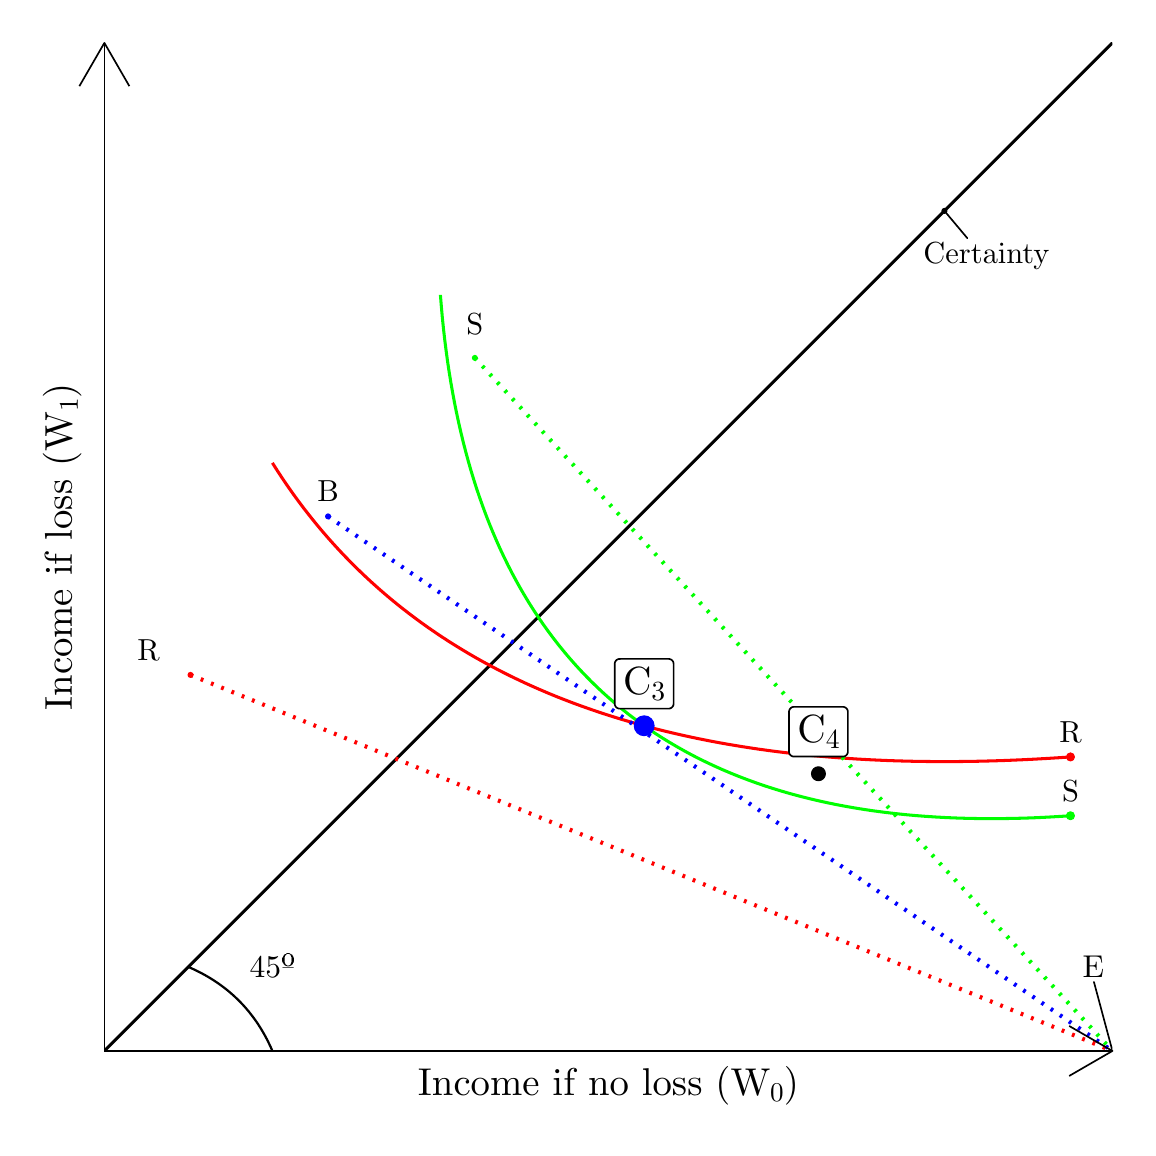
\begin{tikzpicture}[x=1pt,y=1pt]
\definecolor{fillColor}{RGB}{255,255,255}
\path[use as bounding box,fill=fillColor,fill opacity=0.00] (0,0) rectangle (397.48,397.48);
\begin{scope}
\path[clip] (  0.00,  0.00) rectangle (397.48,397.48);
\definecolor{drawColor}{RGB}{255,255,255}
\definecolor{fillColor}{RGB}{255,255,255}

\path[draw=drawColor,line width= 0.6pt,line join=round,line cap=round,fill=fillColor] (  0.00,  0.00) rectangle (397.48,397.48);
\end{scope}
\begin{scope}
\path[clip] ( 27.72, 27.72) rectangle (391.98,391.98);
\definecolor{fillColor}{RGB}{255,255,255}

\path[fill=fillColor] ( 27.72, 27.72) rectangle (391.98,391.98);
\definecolor{drawColor}{RGB}{0,0,0}

\path[draw=drawColor,line width= 1.1pt,line join=round] ( 27.72, 27.72) --
	( 31.40, 31.40) --
	( 35.08, 35.08) --
	( 38.76, 38.76) --
	( 42.44, 42.44) --
	( 46.12, 46.12) --
	( 49.79, 49.79) --
	( 53.47, 53.47) --
	( 57.15, 57.15) --
	( 60.83, 60.83) --
	( 64.51, 64.51) --
	( 68.19, 68.19) --
	( 71.87, 71.87) --
	( 75.55, 75.55) --
	( 79.23, 79.23) --
	( 82.91, 82.91) --
	( 86.59, 86.59) --
	( 90.27, 90.27) --
	( 93.95, 93.95) --
	( 97.63, 97.63) --
	(101.31,101.31) --
	(104.99,104.99) --
	(108.67,108.67) --
	(112.35,112.35) --
	(116.03,116.03) --
	(119.70,119.70) --
	(123.38,123.38) --
	(127.06,127.06) --
	(130.74,130.74) --
	(134.42,134.42) --
	(138.10,138.10) --
	(141.78,141.78) --
	(145.46,145.46) --
	(149.14,149.14) --
	(152.82,152.82) --
	(156.50,156.50) --
	(160.18,160.18) --
	(163.86,163.86) --
	(167.54,167.54) --
	(171.22,171.22) --
	(174.90,174.90) --
	(178.58,178.58) --
	(182.26,182.26) --
	(185.94,185.94) --
	(189.61,189.61) --
	(193.29,193.29) --
	(196.97,196.97) --
	(200.65,200.65) --
	(204.33,204.33) --
	(208.01,208.01) --
	(211.69,211.69) --
	(215.37,215.37) --
	(219.05,219.05) --
	(222.73,222.73) --
	(226.41,226.41) --
	(230.09,230.09) --
	(233.77,233.77) --
	(237.45,237.45) --
	(241.13,241.13) --
	(244.81,244.81) --
	(248.49,248.49) --
	(252.17,252.17) --
	(255.84,255.84) --
	(259.52,259.52) --
	(263.20,263.20) --
	(266.88,266.88) --
	(270.56,270.56) --
	(274.24,274.24) --
	(277.92,277.92) --
	(281.60,281.60) --
	(285.28,285.28) --
	(288.96,288.96) --
	(292.64,292.64) --
	(296.32,296.32) --
	(300.00,300.00) --
	(303.68,303.68) --
	(307.36,307.36) --
	(311.04,311.04) --
	(314.72,314.72) --
	(318.40,318.40) --
	(322.08,322.08) --
	(325.75,325.75) --
	(329.43,329.43) --
	(333.11,333.11) --
	(336.79,336.79) --
	(340.47,340.47) --
	(344.15,344.15) --
	(347.83,347.83) --
	(351.51,351.51) --
	(355.19,355.19) --
	(358.87,358.87) --
	(362.55,362.55) --
	(366.23,366.23) --
	(369.91,369.91) --
	(373.59,373.59) --
	(377.27,377.27) --
	(380.95,380.95) --
	(384.63,384.63) --
	(388.31,388.31) --
	(391.98,391.98);
\definecolor{drawColor}{RGB}{255,0,0}

\path[draw=drawColor,line width= 1.1pt,line join=round] ( 88.43,240.21) --
	( 89.98,237.77) --
	( 91.55,235.36) --
	( 93.15,232.97) --
	( 94.78,230.62) --
	( 96.44,228.29) --
	( 98.13,225.99) --
	( 99.84,223.72) --
	(101.59,221.48) --
	(103.36,219.26) --
	(105.15,217.07) --
	(106.98,214.91) --
	(108.83,212.78) --
	(110.72,210.67) --
	(112.62,208.60) --
	(114.56,206.55) --
	(116.53,204.53) --
	(118.52,202.53) --
	(120.54,200.57) --
	(122.59,198.63) --
	(124.67,196.72) --
	(126.77,194.84) --
	(128.90,192.99) --
	(131.06,191.16) --
	(133.25,189.36) --
	(135.47,187.59) --
	(137.71,185.85) --
	(139.98,184.14) --
	(142.28,182.45) --
	(144.61,180.79) --
	(146.97,179.16) --
	(149.35,177.56) --
	(151.76,175.98) --
	(154.20,174.44) --
	(156.67,172.92) --
	(159.16,171.43) --
	(161.68,169.96) --
	(164.23,168.53) --
	(166.81,167.12) --
	(169.42,165.74) --
	(172.05,164.39) --
	(174.72,163.06) --
	(177.41,161.77) --
	(180.12,160.50) --
	(182.87,159.26) --
	(185.64,158.05) --
	(188.44,156.86) --
	(191.27,155.70) --
	(194.13,154.58) --
	(197.02,153.47) --
	(199.93,152.40) --
	(202.87,151.36) --
	(205.84,150.34) --
	(208.83,149.35) --
	(211.86,148.39) --
	(214.91,147.45) --
	(217.99,146.55) --
	(221.10,145.67) --
	(224.23,144.82) --
	(227.40,144.00) --
	(230.59,143.20) --
	(233.81,142.44) --
	(237.06,141.70) --
	(240.33,140.99) --
	(243.64,140.30) --
	(246.97,139.65) --
	(250.33,139.02) --
	(253.71,138.42) --
	(257.13,137.85) --
	(260.57,137.31) --
	(264.04,136.79) --
	(267.54,136.30) --
	(271.06,135.84) --
	(274.62,135.41) --
	(278.20,135.01) --
	(281.81,134.63) --
	(285.45,134.28) --
	(289.11,133.96) --
	(292.81,133.67) --
	(296.53,133.41) --
	(300.28,133.17) --
	(304.05,132.96) --
	(307.86,132.78) --
	(311.69,132.62) --
	(315.55,132.50) --
	(319.44,132.40) --
	(323.36,132.33) --
	(327.30,132.29) --
	(331.27,132.28) --
	(335.27,132.29) --
	(339.30,132.33) --
	(343.36,132.40) --
	(347.44,132.50) --
	(351.55,132.62) --
	(355.69,132.78) --
	(359.86,132.96) --
	(364.05,133.17) --
	(368.28,133.41) --
	(372.53,133.67) --
	(376.81,133.96);
\definecolor{drawColor}{RGB}{0,255,0}

\path[draw=drawColor,line width= 1.1pt,line join=round] (149.14,300.92) --
	(149.47,296.83) --
	(149.83,292.79) --
	(150.24,288.79) --
	(150.69,284.84) --
	(151.18,280.93) --
	(151.70,277.07) --
	(152.27,273.25) --
	(152.88,269.48) --
	(153.53,265.75) --
	(154.22,262.06) --
	(154.95,258.42) --
	(155.72,254.82) --
	(156.53,251.27) --
	(157.38,247.77) --
	(158.27,244.30) --
	(159.20,240.89) --
	(160.17,237.51) --
	(161.18,234.19) --
	(162.23,230.90) --
	(163.33,227.66) --
	(164.46,224.47) --
	(165.63,221.32) --
	(166.84,218.21) --
	(168.10,215.15) --
	(169.39,212.14) --
	(170.72,209.17) --
	(172.10,206.24) --
	(173.51,203.36) --
	(174.96,200.52) --
	(176.46,197.73) --
	(177.99,194.98) --
	(179.57,192.27) --
	(181.18,189.61) --
	(182.84,187.00) --
	(184.53,184.43) --
	(186.27,181.90) --
	(188.05,179.42) --
	(189.86,176.99) --
	(191.72,174.60) --
	(193.62,172.25) --
	(195.55,169.95) --
	(197.53,167.69) --
	(199.55,165.47) --
	(201.61,163.31) --
	(203.71,161.18) --
	(205.84,159.10) --
	(208.02,157.07) --
	(210.24,155.08) --
	(212.50,153.13) --
	(214.80,151.23) --
	(217.14,149.37) --
	(219.52,147.56) --
	(221.94,145.80) --
	(224.40,144.07) --
	(226.90,142.39) --
	(229.44,140.76) --
	(232.03,139.17) --
	(234.65,137.63) --
	(237.31,136.13) --
	(240.01,134.67) --
	(242.75,133.26) --
	(245.54,131.90) --
	(248.36,130.58) --
	(251.22,129.30) --
	(254.13,128.07) --
	(257.07,126.88) --
	(260.06,125.74) --
	(263.08,124.64) --
	(266.14,123.58) --
	(269.25,122.58) --
	(272.39,121.61) --
	(275.58,120.69) --
	(278.81,119.82) --
	(282.07,118.99) --
	(285.38,118.20) --
	(288.72,117.46) --
	(292.11,116.76) --
	(295.54,116.11) --
	(299.01,115.50) --
	(302.51,114.94) --
	(306.06,114.42) --
	(309.65,113.95) --
	(313.28,113.52) --
	(316.95,113.13) --
	(320.66,112.79) --
	(324.40,112.50) --
	(328.19,112.25) --
	(332.02,112.04) --
	(335.89,111.88) --
	(339.80,111.76) --
	(343.75,111.69) --
	(347.74,111.66) --
	(351.78,111.68) --
	(355.85,111.74) --
	(359.96,111.84) --
	(364.11,111.99) --
	(368.30,112.19) --
	(372.53,112.43) --
	(376.81,112.71);
\definecolor{drawColor}{RGB}{0,0,255}
\definecolor{fillColor}{RGB}{0,0,255}

\path[draw=drawColor,line width= 0.4pt,line join=round,line cap=round,fill=fillColor] (222.77,145.22) circle (  3.57);
\definecolor{drawColor}{RGB}{0,0,0}
\definecolor{fillColor}{RGB}{255,255,255}

\path[draw=drawColor,line width= 0.6pt,line join=round,line cap=round,fill=fillColor] (213.94,151.41) --
	(231.60,151.41) --
	(231.52,151.41) --
	(231.81,151.43) --
	(232.10,151.48) --
	(232.37,151.59) --
	(232.62,151.73) --
	(232.85,151.92) --
	(233.04,152.13) --
	(233.20,152.38) --
	(233.31,152.65) --
	(233.38,152.93) --
	(233.40,153.22) --
	(233.40,153.22) --
	(233.40,167.57) --
	(233.40,167.57) --
	(233.38,167.86) --
	(233.31,168.14) --
	(233.20,168.41) --
	(233.04,168.66) --
	(232.85,168.88) --
	(232.62,169.06) --
	(232.37,169.20) --
	(232.10,169.31) --
	(231.81,169.37) --
	(231.60,169.38) --
	(213.94,169.38) --
	(214.15,169.37) --
	(213.86,169.38) --
	(213.57,169.34) --
	(213.29,169.26) --
	(213.03,169.14) --
	(212.79,168.97) --
	(212.58,168.77) --
	(212.41,168.54) --
	(212.27,168.28) --
	(212.18,168.00) --
	(212.13,167.72) --
	(212.13,167.57) --
	(212.13,153.22) --
	(212.13,153.36) --
	(212.13,153.07) --
	(212.18,152.79) --
	(212.27,152.51) --
	(212.41,152.25) --
	(212.58,152.02) --
	(212.79,151.82) --
	(213.03,151.65) --
	(213.29,151.53) --
	(213.57,151.45) --
	(213.86,151.41) --
	cycle;
\end{scope}
\begin{scope}
\path[clip] ( 27.72, 27.72) rectangle (391.98,391.98);
\definecolor{drawColor}{RGB}{0,0,0}

\node[text=drawColor,anchor=base west,inner sep=0pt, outer sep=0pt, scale=  1.42] at (215.14,156.57) {C};

\node[text=drawColor,anchor=base west,inner sep=0pt, outer sep=0pt, scale=  1.00] at (225.41,154.42) {3};
\definecolor{drawColor}{RGB}{255,0,0}

\path[draw=drawColor,line width= 1.5pt,dash pattern=on 1pt off 3pt ,line join=round] ( 58.83,163.59) --
	(391.98, 27.72);
\definecolor{drawColor}{RGB}{0,255,0}

\path[draw=drawColor,line width= 1.5pt,dash pattern=on 1pt off 3pt ,line join=round] (161.59,278.15) --
	(391.98, 27.72);
\definecolor{drawColor}{RGB}{0,0,255}

\path[draw=drawColor,line width= 1.5pt,dash pattern=on 1pt off 3pt ,line join=round] (108.54,220.87) --
	(391.98, 27.72);
\definecolor{drawColor}{RGB}{255,0,0}
\definecolor{fillColor}{RGB}{255,0,0}

\path[draw=drawColor,line width= 0.4pt,line join=round,line cap=round,fill=fillColor] ( 58.83,163.59) circle (  0.89);
\definecolor{drawColor}{RGB}{0,0,0}

\node[text=drawColor,anchor=base,inner sep=0pt, outer sep=0pt, scale=  1.10] at ( 43.65,168.89) {R};
\definecolor{drawColor}{RGB}{0,255,0}
\definecolor{fillColor}{RGB}{0,255,0}

\path[draw=drawColor,line width= 0.4pt,line join=round,line cap=round,fill=fillColor] (161.59,278.15) circle (  0.89);
\definecolor{drawColor}{RGB}{0,0,0}

\node[text=drawColor,anchor=base,inner sep=0pt, outer sep=0pt, scale=  1.10] at (161.59,286.49) {S};
\definecolor{drawColor}{RGB}{0,0,255}
\definecolor{fillColor}{RGB}{0,0,255}

\path[draw=drawColor,line width= 0.4pt,line join=round,line cap=round,fill=fillColor] (108.54,220.87) circle (  0.89);
\definecolor{drawColor}{RGB}{0,0,0}

\node[text=drawColor,anchor=base,inner sep=0pt, outer sep=0pt, scale=  1.10] at (108.54,226.18) {B};

\path[draw=drawColor,line width= 0.8pt,line join=round] ( 58.07, 58.07) --
	( 58.50, 57.89) --
	( 58.93, 57.70) --
	( 59.35, 57.51) --
	( 59.77, 57.32) --
	( 60.19, 57.12) --
	( 60.60, 56.93) --
	( 61.02, 56.73) --
	( 61.43, 56.52) --
	( 61.84, 56.32) --
	( 62.24, 56.11) --
	( 62.65, 55.90) --
	( 63.05, 55.69) --
	( 63.44, 55.47) --
	( 63.84, 55.26) --
	( 64.23, 55.04) --
	( 64.62, 54.81) --
	( 65.01, 54.59) --
	( 65.40, 54.36) --
	( 65.78, 54.13) --
	( 66.16, 53.90) --
	( 66.54, 53.66) --
	( 66.92, 53.43) --
	( 67.29, 53.19) --
	( 67.66, 52.94) --
	( 68.03, 52.70) --
	( 68.40, 52.45) --
	( 68.76, 52.20) --
	( 69.12, 51.95) --
	( 69.48, 51.70) --
	( 69.84, 51.44) --
	( 70.19, 51.18) --
	( 70.54, 50.92) --
	( 70.89, 50.65) --
	( 71.24, 50.39) --
	( 71.58, 50.12) --
	( 71.92, 49.85) --
	( 72.26, 49.57) --
	( 72.60, 49.29) --
	( 72.93, 49.01) --
	( 73.26, 48.73) --
	( 73.59, 48.45) --
	( 73.92, 48.16) --
	( 74.24, 47.87) --
	( 74.56, 47.58) --
	( 74.88, 47.29) --
	( 75.20, 46.99) --
	( 75.51, 46.69) --
	( 75.82, 46.39) --
	( 76.13, 46.08) --
	( 76.44, 45.78) --
	( 76.74, 45.47) --
	( 77.05, 45.16) --
	( 77.34, 44.84) --
	( 77.64, 44.53) --
	( 77.94, 44.21) --
	( 78.23, 43.89) --
	( 78.52, 43.56) --
	( 78.80, 43.24) --
	( 79.09, 42.91) --
	( 79.37, 42.58) --
	( 79.65, 42.24) --
	( 79.93, 41.91) --
	( 80.20, 41.57) --
	( 80.47, 41.22) --
	( 80.74, 40.88) --
	( 81.01, 40.53) --
	( 81.27, 40.19) --
	( 81.54, 39.83) --
	( 81.80, 39.48) --
	( 82.05, 39.13) --
	( 82.31, 38.77) --
	( 82.56, 38.41) --
	( 82.81, 38.04) --
	( 83.06, 37.68) --
	( 83.30, 37.31) --
	( 83.54, 36.94) --
	( 83.78, 36.56) --
	( 84.02, 36.19) --
	( 84.25, 35.81) --
	( 84.49, 35.43) --
	( 84.72, 35.04) --
	( 84.94, 34.66) --
	( 85.17, 34.27) --
	( 85.39, 33.88) --
	( 85.61, 33.49) --
	( 85.83, 33.09) --
	( 86.04, 32.69) --
	( 86.26, 32.29) --
	( 86.47, 31.89) --
	( 86.67, 31.48) --
	( 86.88, 31.07) --
	( 87.08, 30.66) --
	( 87.28, 30.25) --
	( 87.48, 29.83) --
	( 87.67, 29.42) --
	( 87.87, 28.99) --
	( 88.06, 28.57) --
	( 88.24, 28.15) --
	( 88.43, 27.72);

\node[text=drawColor,anchor=base,inner sep=0pt, outer sep=0pt, scale=  1.14] at ( 88.43, 54.15) {45º};

\path[draw=drawColor,line width= 0.6pt,line join=round,line cap=round] (385.29, 52.65) -- (391.98, 27.72);

\node[text=drawColor,anchor=base,inner sep=0pt, outer sep=0pt, scale=  1.14] at (385.10, 54.15) {E};
\definecolor{fillColor}{RGB}{0,0,0}

\path[draw=drawColor,line width= 0.4pt,line join=round,line cap=round,fill=fillColor] (285.74,127.89) circle (  2.50);
\definecolor{fillColor}{RGB}{255,255,255}

\path[draw=drawColor,line width= 0.6pt,line join=round,line cap=round,fill=fillColor] (276.91,134.09) --
	(294.57,134.09) --
	(294.50,134.09) --
	(294.79,134.10) --
	(295.07,134.16) --
	(295.35,134.26) --
	(295.60,134.41) --
	(295.82,134.59) --
	(296.02,134.81) --
	(296.17,135.05) --
	(296.29,135.32) --
	(296.35,135.60) --
	(296.38,135.89) --
	(296.38,135.89) --
	(296.38,150.25) --
	(296.38,150.25) --
	(296.35,150.54) --
	(296.29,150.82) --
	(296.17,151.09) --
	(296.02,151.33) --
	(295.82,151.55) --
	(295.60,151.73) --
	(295.35,151.88) --
	(295.07,151.98) --
	(294.79,152.04) --
	(294.57,152.05) --
	(276.91,152.05) --
	(277.13,152.04) --
	(276.84,152.05) --
	(276.55,152.02) --
	(276.27,151.94) --
	(276.01,151.81) --
	(275.77,151.65) --
	(275.56,151.44) --
	(275.38,151.21) --
	(275.25,150.95) --
	(275.16,150.68) --
	(275.11,150.39) --
	(275.10,150.25) --
	(275.10,135.89) --
	(275.11,136.04) --
	(275.11,135.75) --
	(275.16,135.46) --
	(275.25,135.18) --
	(275.38,134.93) --
	(275.56,134.69) --
	(275.77,134.49) --
	(276.01,134.33) --
	(276.27,134.20) --
	(276.55,134.12) --
	(276.84,134.09) --
	cycle;
\end{scope}
\begin{scope}
\path[clip] ( 27.72, 27.72) rectangle (391.98,391.98);
\definecolor{drawColor}{RGB}{0,0,0}

\node[text=drawColor,anchor=base west,inner sep=0pt, outer sep=0pt, scale=  1.42] at (278.11,139.24) {C};

\node[text=drawColor,anchor=base west,inner sep=0pt, outer sep=0pt, scale=  1.00] at (288.39,137.10) {4};
\definecolor{drawColor}{RGB}{255,0,0}
\definecolor{fillColor}{RGB}{255,0,0}

\path[draw=drawColor,line width= 0.4pt,line join=round,line cap=round,fill=fillColor] (376.81,133.96) circle (  1.43);
\definecolor{drawColor}{RGB}{0,0,0}

\node[text=drawColor,anchor=base,inner sep=0pt, outer sep=0pt, scale=  1.10] at (376.81,139.27) {R};
\definecolor{drawColor}{RGB}{0,255,0}
\definecolor{fillColor}{RGB}{0,255,0}

\path[draw=drawColor,line width= 0.4pt,line join=round,line cap=round,fill=fillColor] (376.81,112.71) circle (  1.43);
\definecolor{drawColor}{RGB}{0,0,0}

\node[text=drawColor,anchor=base,inner sep=0pt, outer sep=0pt, scale=  1.10] at (376.81,118.02) {S};
\definecolor{fillColor}{RGB}{0,0,0}

\path[draw=drawColor,line width= 0.4pt,line join=round,line cap=round,fill=fillColor] (331.27,331.27) circle (  0.89);

\path[draw=drawColor,line width= 0.6pt,line join=round,line cap=round] (339.55,321.40) -- (331.27,331.27);

\node[text=drawColor,anchor=base,inner sep=0pt, outer sep=0pt, scale=  1.10] at (346.45,312.29) {Certainty};
\end{scope}
\begin{scope}
\path[clip] (  0.00,  0.00) rectangle (397.48,397.48);
\definecolor{drawColor}{RGB}{0,0,0}

\path[draw=drawColor,line width= 0.6pt,line join=round] ( 27.72, 27.72) --
	( 27.72,391.98);

\path[draw=drawColor,line width= 0.6pt,line join=round] ( 36.75,376.34) --
	( 27.72,391.98) --
	( 18.68,376.34);
\end{scope}
\begin{scope}
\path[clip] (  0.00,  0.00) rectangle (397.48,397.48);
\definecolor{drawColor}{RGB}{0,0,0}

\path[draw=drawColor,line width= 0.6pt,line join=round] ( 27.72, 27.72) --
	(391.98, 27.72);

\path[draw=drawColor,line width= 0.6pt,line join=round] (376.34, 18.68) --
	(391.98, 27.72) --
	(376.34, 36.75);
\end{scope}
\begin{scope}
\path[clip] (  0.00,  0.00) rectangle (397.48,397.48);
\definecolor{drawColor}{RGB}{0,0,0}

\node[text=drawColor,anchor=base west,inner sep=0pt, outer sep=0pt, scale=  1.40] at (141.04, 11.72) {Income if no loss (W};

\node[text=drawColor,anchor=base west,inner sep=0pt, outer sep=0pt, scale=  0.98] at (268.33,  9.61) {0};

\node[text=drawColor,anchor=base west,inner sep=0pt, outer sep=0pt, scale=  1.40] at (273.22, 11.72) {)};
\end{scope}
\begin{scope}
\path[clip] (  0.00,  0.00) rectangle (397.48,397.48);
\definecolor{drawColor}{RGB}{0,0,0}

\node[text=drawColor,rotate= 90.00,anchor=base west,inner sep=0pt, outer sep=0pt, scale=  1.40] at ( 16.00,150.76) {Income if loss (W};

\node[text=drawColor,rotate= 90.00,anchor=base west,inner sep=0pt, outer sep=0pt, scale=  0.98] at ( 18.11,258.61) {1};

\node[text=drawColor,rotate= 90.00,anchor=base west,inner sep=0pt, outer sep=0pt, scale=  1.40] at ( 16.00,263.50) {)};
\end{scope}
\end{tikzpicture}
